\chapter{Related Work}
In this section we will examine some popular data extraction tools and describe their usage and their benefits along with their drawback. We will present a very popular browser extension named Selenium (\url{http://www.seleniumhq.org/}) to illustrate the state-of-the-art software for browser automaton, then we will inspect 3 different scrapers. First of them, iOpus (\url{http://imacros.net/}), is the most popular browser extension, used for scraping, having over 10 milion downloads, then we will look at Deixto\cite{kokkoras2013deixto}, which is a very popular free software. Then we will describe languages based on extending the XPath language, namely OXPath ans SXPath  and last we will inspect the most popular commercial solution, Lixto\cite{baumgartner2001visual}, which is a GUI around the Elog language.

Because GUI is just a mere wrapper around the language and~it reflects the~strengths and~weaknesses of~the~languages, we will pay most attention to the language.


\section{Selenium}
Selenium (\url{http://www.seleniumhq.org/}) is self-described with a statement \textit{Selenium automates browsers. That's it!} which is an accurate description. Although this tool is not a Web Data Extraction system per se, it shares almost all attributes with them. Moreover, Selenium offers two services, Selenium IDE, which is a browser extension and Selenium WebDriver, which is a collection of bindings to programming languages, so that the user will be able to work with the data after processing.
Nevertheless, the main selling point of the product is testing and automation, i.e. writing automated tests for a web service.

Users can either write custom macros that consist of a list of commands to be executed, or simply press the "Start recording" button and manually perform the actions in the browser. The extension will record the action and generate a wrapper.

Apart from basic commands for navigation, such as filling out the forms, clicking on the buttons and following the links, it is also equipped with testing related functionality, like asserts for a concrete value in a given selector.

This tool provides front-end web testers with unparalleled services to the point that it has become a de facto standard in the web testing stack.

Although the language is fully-equipped for navigation and automation, it lacks in other areas, e.g. it does not provide a mean to transform the extracted data, or to edit the DOM - this functionality is further delegated.

The web-driver wrapper around the language is available in multiple languages, however, it  still does not provide any data transformation capabilities.

\subsection{Example}
We examined this tool by a real-world example, where we logged into Facebook and selected the second most recent conversation.
Source of the macro is in figure~\ref{fig:seleniumCommands}
\begin{figure}
    \centering
    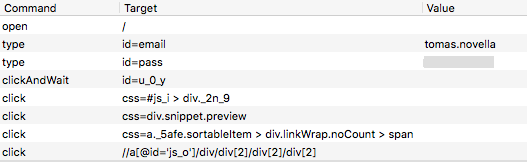
\includegraphics[width=\textwidth]{../img/seleniumCommands}
    \caption{A series of commands that leads to logging into \url{https://www.facebook.com} and choosing the second most recent conversation}
    \label{fig:seleniumCommands}
\end{figure}

\section{iMacros}
This tool, formerly known as iOpus, strongly resembles the Selenium IDE and is in fact targeting a very similar audience. It even provides a website that lists the distinctions between iMacros and Selenium (\url{http://wiki.imacros.net/Selenium}). The use cases differ from Selenium and are as follows:
\begin{enumerate}
    \item Browser Automation
    \item Web Testing
    \item Data Extraction
\end{enumerate}

\subsection{Browser Automation and Web Testing}
In these areas is the tool very similar to Selenium. Form filling and link navigation are standard and 
The command set is very similar, only has different names.
Moreover, it offers a possibility to extract data into variables and to navigate through more complex dynamic pages, supporting sliders (\url{http://maps.google.com}) and drag-and-drop functionality.
Identification of the elements on the page is either by XPath, CSS selectors, or by the element's type, positions and attributes. On top of this, is offers functionality to detect and intercept built-in browser dialogs, such as the download dialog and native Javascript dialogs. A very nice advanced functionality is the image recognition functionality. It relies on the rendering of the image and using advanced neural networks it can identify the element, even if it has moved, or has changed color.

\subsection{Data Extraction}
This is the main differentiator; in this domain, we can select a variable to which the data will be extracted. Plain-text and CSV output formats are supported.
One of the most significant drawbacks is the lack of any structure in the extracted data, it is a simple flat list of data.

\subsection{Example}
Again, we tried to log into Facebook and select the second conversation. Automatic recording broke down, but after some manual effort we made a macro in Figure \ref{fig:iMacrosCommands}.
\begin{figure}
    \centering
    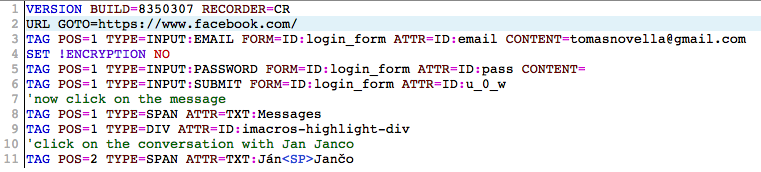
\includegraphics[width=\textwidth]{../img/iMacrosCommands}
    \caption{A series of commands that leads to logging into \url{https://www.facebook.com} and choosing a conversation with Jan Janco.}
    \label{fig:iMacrosCommands}
\end{figure}


\section{XPath-based languages}
In this section we
\subsection{OXPath}
\subsection{SXPath}

\section{Deixto}

\section{Lixto}
